% !TeX root = ../../thesis.tex
\chapter{From Perovskite Films to Photodetectors: Establishing a Baseline}\label{ch:material_properties}


The beginning of this work is signified by the transition to a new evaporator chamber by Lesker. 

Goal of this chapter is to give the reader a broad understanding a broad understanding of the various parameters that can be tuned during the fabrication of the perovskite-based photodetectors. 

Perovskite are known for their defect tolerant structure, this means that variation from the perfect stoichiometry do not have a negative impact on the performance of the device. This has an opposite effect at the same time, that despite pursuing changes in the compsosition and the fabrication does not translate to a major impact on the the device peroformance. The first part regards the deposition of the peorovskite thin film and the characterization of its quality before and after annealing via a varierty of measurements, including UV-Vis, Photoluminescence, GIWAXS, as well as morphology through SEM and AFM. 

In the second chapter, we start using this films to investigate the development of photodetector devices. After introducing the structure and the combinations of transportl layer we can use, we indeintify the drastic impact of the characterization protocol on the peroformance itself. We end up to a convention that will be used for the characterization of the devices from now onwards. 

This way we proceed on presenting the baseline device architecture, including the choice of transport layers, the total deposition rate, and the samples stoichiometry. We close the chapter by introducing the silicon substrate that matches closer the substrate for the development of imagers, introducing the main differences and characteristics of the performance. 



\section{Perovskite Deposition}



\begin{figure}
  \centering
  \medskip
  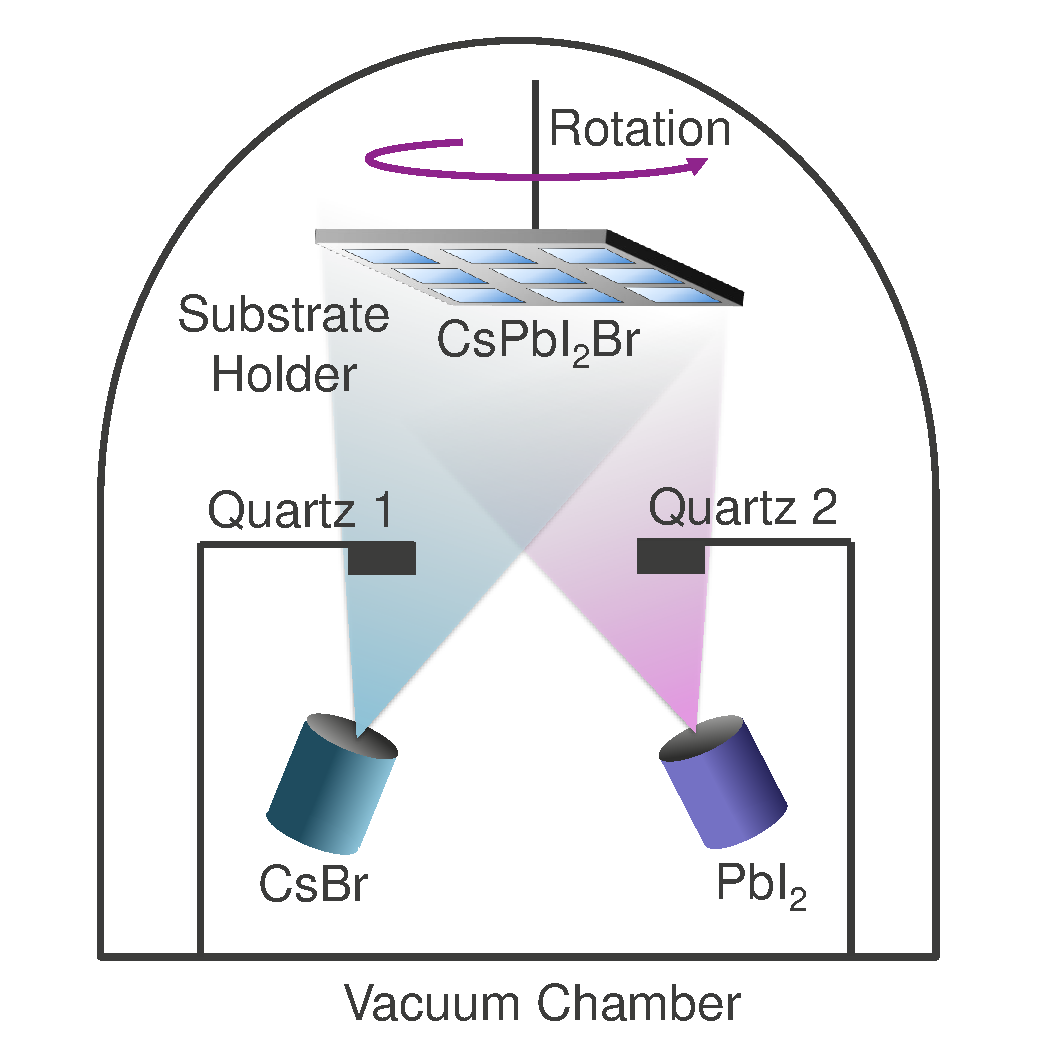
\includegraphics[width=.5\textwidth]{chapters/material_properties/images/Chamber.pdf}
  \caption[Short caption for Table of Figures]{Illustration of the deposition chamber. Two diametrically opposed sources are used for CsBr and PbI2.}
  \label{fig:deposition_chamber}
\end{figure}



\begin{itemize}
    \item Visual icon of the co-evaporation chamber and explanation of parts + add icon of the substrate holder
    \item Sources and calibration of tooling factor - evaporation rates through spectroscopic ellipsometry (add plots that show the fitting and the average)
    \item Selection of co-evaporation rate/ratio and why
\end{itemize}

An illustration of the deposition chamber is provided in Figure~\ref{fig:deposition_chamber}. Two diametrically opposed sources are loaded with CsBr and PbI2 powders, respectively. It was found that the replacement of fresh powders can help endure a more unfirm deposition, comparing the XRD spectra of fresh powders, and the powders post deposition. 


Two separate quartz monitors are used to monitor the deposition rate of each source. 

The quartz monitors need to be calibrated according to the atomic mass of the precursor, whose deposition rate they are supposed to be monitoring. 

To do that, an initial approximation of the estimated tooling factor based on comparisons with previous deposition need to be made. 

Afterwards, multiple depositions of each precursor are made on silicon substrate. 

The thickeness of the deposited layer is measured using spectroscopic ellipsometry. 

The tooling factor is adjusted according to the equation TFfinal = Tfinitial thickness(estimated)/thickness(real). 

We deposit the layer mutliple times at different rates and different target thicknesses, to account for variablity in the system The finlan tooling factor is calculated as the average of the alla attempts. 

This allows for the starting of the co-evaporation, were both rates are controlled simultaneously. While the sources are heatigng up, a global shutter is protecting the samples from the deposition

Once the rates of both samples have reached the target value and are stabilized, the shutter opens and the deposition is started. 

The substrate holder, which can be loaded with 9 3 by 3 cm2 samples, was kept at room temperature and was rotating with 5 rounds per minute to ensure a smoother deposition. 

During the deposition, the temperature was automatically increased to maintain a constatnt evaporation rate for both sources. 

When the target thickness was reached, the global shutter was closed, and the sources were cooled down to room temp. 



\subsection{Impact of Annealing on Material Properties}

This chapter explores the impact of annealing on the material properties of the as-deposited film. 

Figure 2.2 compared the morphology of an as-deposited and annealed sample. The as-deposited sample has grain size in the rage of of xx to yy nm. 

The film is compact with no visible cracks, piholes, or areas with varied stoichiometry.

Once the sample is annealed, the averga grain size increases to approxiamtely 100 nm, followed by a significant increase in surface roughness, from 2 nm to 28.5 nm. 

This is translated in the optoelctronic properties of the films. When comparing the absoloute intensity, a 3 times increase in the PL siganl is observed for the annealed perovskite. Exciation of wavelngths is 560 nm

Fig. x compared the absorptance of the film. An additional increase of the absorptance at the spectrum beyond 500 nm is oncersver. At 560 nm, the excitation wvl of PL,  an increase from 71\% to 74\% is observed, which means that the incerase in PL intensity can not be solely attributed to the increase of the absorpatace. Contrary, it points out to imporved crystallinity and reduction of recombination centers. When comparing the normalized PL peaks, an additional change os observed, a shoulder in the peak is observed for the Annealed state. Wider FWHM is sually attribure to lower quality, however this kind of non-symmetrical broadedning was previously attribute to the self-absorbing mechanisms,close to the bandgap energy, followed by re-emission. this mechanism is exaggerated by internal light scattering, which matches with increase surfae roughness of the films. 

Lastly, Fig. xx shoes the transient state photoluminescence of the films, indicating a doubling of the lifetime of the carriers from 4.8 for the as-deposited state to 8.3 nm for the annealed state. 

To further investigate the crystallility and phsae transition temperature of the perovskite we further submitted the samples to in situ GIWAXS measuremernts. Fig. 2.5 compares the crystalline structure for the as-deposited and annealed state at room temperature. The as-deposited can be purely described by the considertation of the gamma CsPbI2Br phase, highlighting the ability of the perovskite to produce ttabtle films in the balck phase without any need for additional heating. This was widely investigatef FOR CsPbI3 films, but with a heated substrate. The ability to produde black film without any heat could open up a completly new realm of opeerations, such as flexible substrates that have very low temperature limiationts. 

The crystalline peaks for the annealed state, reveal more informaiton aobut the strucutre of the film. The peaks are separeatedand additional peaks, more clearly notices at 9 nm-1 is obsefved. Thsi indicaated an increase in crystallite size, while at the same time incease stress in the lattice, the presence of the 0D Cs4PbI2Br2. However, the oD phase cannot be detected in the absorptance signal pf the perovsite (high bandgap) as it was shown that it only appears for very high difference between the two precursors.  

In situ measurement can provide more information about the phase transition temperatures and the point of emergence for the Specifically, it is indicated that the orthorhombic to tetragonal phase transition is achieved at 130C, while the tetragona to cubic is accomplished at 190C. The 0D phase is energing at 225C.



\begin{figure}[htbp]
    \centering
    % First row
    \begin{subfigure}[t]{0.45\textwidth}
        \centering
        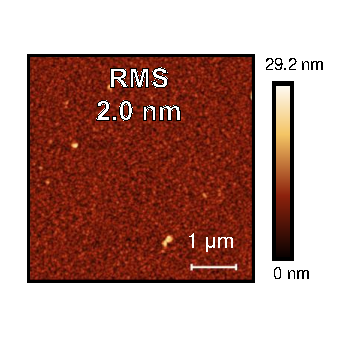
\includegraphics[width=\textwidth]{chapters/material_properties/images/AFM_before.pdf} 
        \caption{}
        \label{fig:ch2:afm_before}
    \end{subfigure}
    \hfill
    \begin{subfigure}[t]{0.45\textwidth}
        \centering
        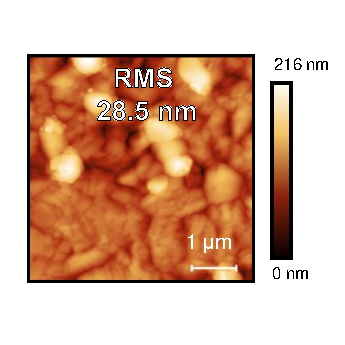
\includegraphics[width=\textwidth]{chapters/material_properties/images/AFM_after.pdf} % Replace with your image file        
        \caption{}
        \label{fig:ch2:afm_after}
    \end{subfigure}

    \vspace{1em} % Space between rows

    % Second row
    \begin{subfigure}[t]{0.4\textwidth}
        \centering
        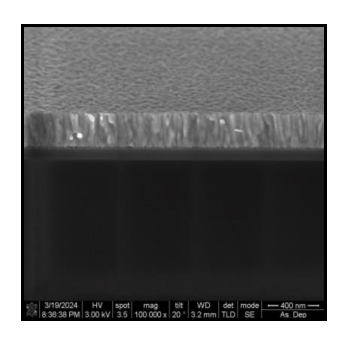
\includegraphics[width=\textwidth]{chapters/material_properties/images/SEM_Before.pdf} 
        \caption{}
        \label{fig:ch2:sem_before}
    \end{subfigure}
    \hfill
    \begin{subfigure}[t]{0.4\textwidth}
        \centering
        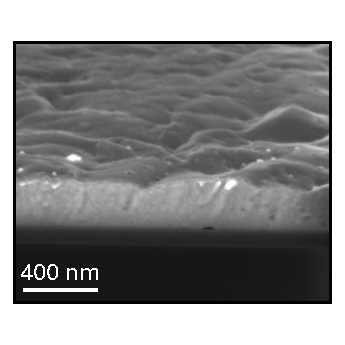
\includegraphics[width=\textwidth]{chapters/material_properties/images/SEM_After.pdf} 
        \caption{}
        \label{fig:ch2:sem_after}
    \end{subfigure}
    \caption{AFM and SEM iamges for an as-deposited and annealed perovskite sample.}
    \label{fig:ch2:afm_sem}
\end{figure}


\begin{figure}[htbp]
    \centering
    % First row
    \begin{subfigure}[t]{0.45\textwidth}
        \centering
        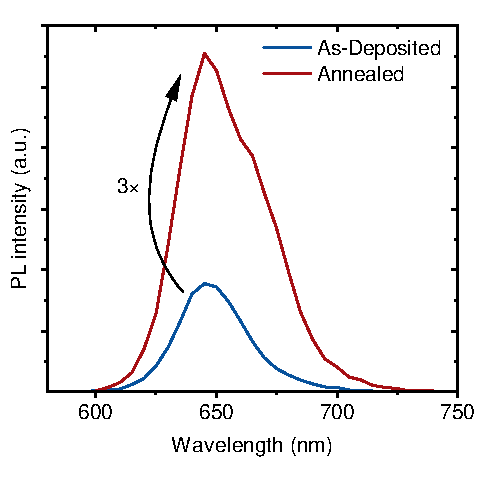
\includegraphics[width=\textwidth]{chapters/material_properties/images/SSPL.pdf} 
        \caption{}
        \label{fig:ch2:sspl}
    \end{subfigure}
    \hfill
    \begin{subfigure}[t]{0.45\textwidth}
        \centering
        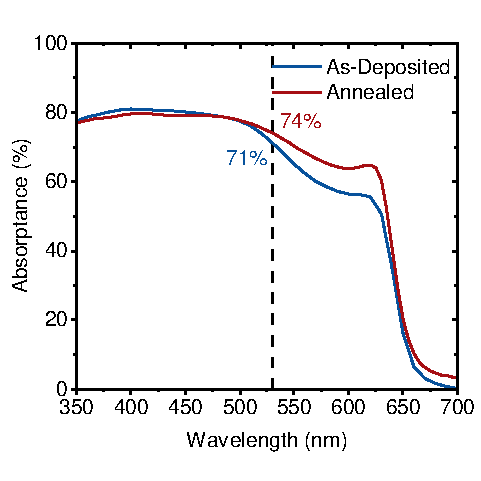
\includegraphics[width=\textwidth]{chapters/material_properties/images/Absorptance.pdf} % Replace with your image file
        \caption{}
        \label{fig:ch2:absorptance}
    \end{subfigure}

    \vspace{1em} % Space between rows

    % Second row
    \begin{subfigure}[t]{0.45\textwidth}
        \centering
        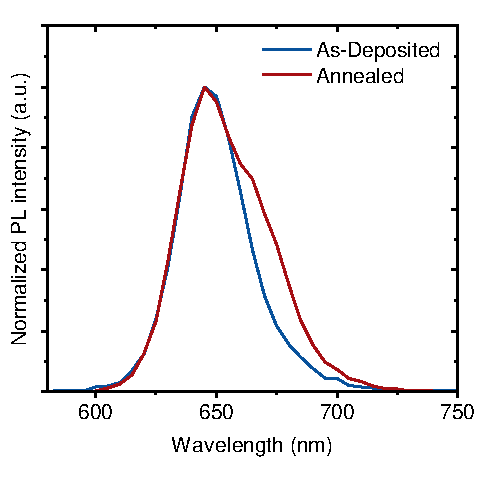
\includegraphics[width=\textwidth]{chapters/material_properties/images/SSPL_norm.pdf} % Replace with your image file
        \caption{}
        \label{fig:ch2:norm_sspl}
    \end{subfigure}
    \hfill
    \begin{subfigure}[t]{0.45\textwidth}
        \centering
        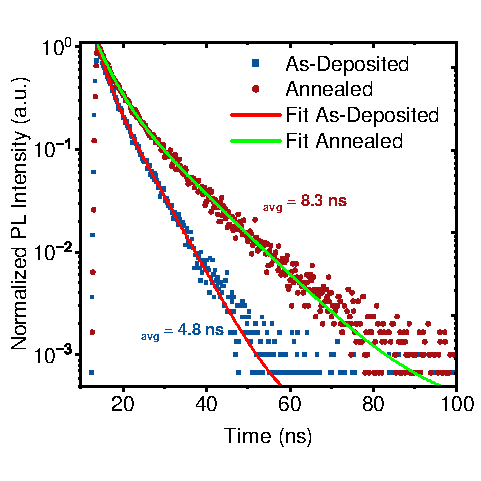
\includegraphics[width=\textwidth]{chapters/material_properties/images/TRPL_norm_double - Copy.pdf} % Replace with your image file
        \caption{}
        \label{fig:ch2:trpl}
    \end{subfigure}
    \caption{SSPL, TRPL, and absorptance for the an As-Deposited and an Annealed perovskite sample.}
\end{figure}

\begin{figure}
  \centering
  \medskip
  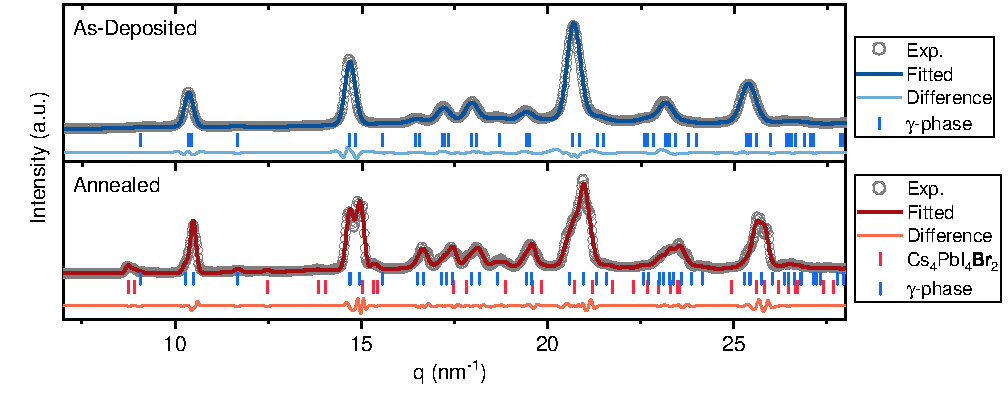
\includegraphics[width=\textwidth]{chapters/material_properties/images/GIWAXS_Before_After.pdf}
  \caption[Short caption for Table of Figures]{In Situ GIWAXS}
  \label{fig:ch2:giwaxs_before_after}
\end{figure}


% % Some dummy code show how to include images.
\begin{figure}
  \centering
  \medskip
  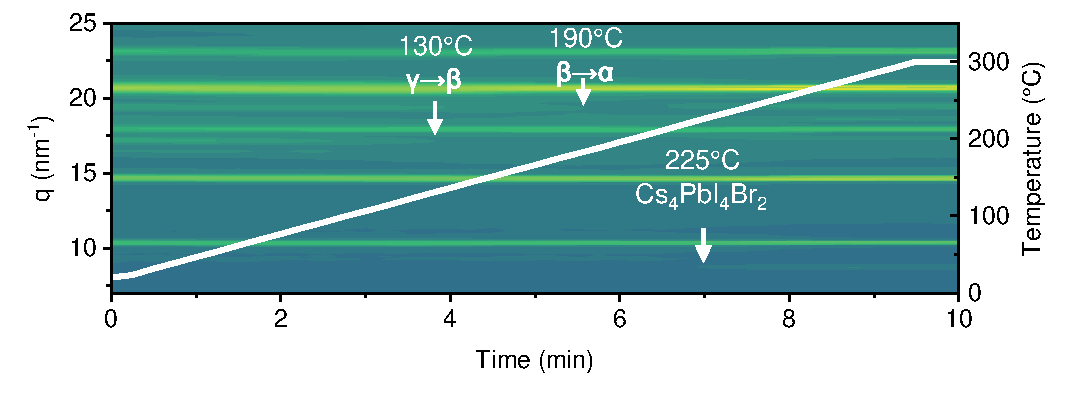
\includegraphics[width=\textwidth]{chapters/material_properties/images/GIWAXS_In_Situ.pdf}
  \caption[Short caption for Table of Figures]{In Situ GIWAXS}
  \label{fig:ch2:giwaxs_insitu}
\end{figure}

\begin{itemize}
    \item Characterization of as-deposited and annealed films via AFM, SEM, SSPL, TRPL, aborptance/reflectance measurements, XPS/UPS
    \item In situ characterization through in situ, temperature dependent GIWAXS, phase identification, phase transition identification, 0-D phase emergence, crystallite size etc
\end{itemize}

\section{Device Development}

Main focus is on the use of thermally evaporated perovskite for photodetector devices. The structure is similar to what has been ued for solar cell fabrication, as explained in the introduction chapter. Two types of substrates are used. For fat prototyping, glass substrate with pre-patterned ITO contacts, sequential deposition of the hole transport layer, the perovskite, the electronc transport layer and the top contact. The illumination is down from the glass size. 

An alterntiave silicon substrate is used for the same stack, which is more similaer to the strucutre os the imager. Silicon substrate with SiO2 dielectric, and TiN Bbottm electrodes (which define the area of the device). The stack is built in the same way, HTL, perovskite, ETL. ITO is deposited dual purpose, serves as the common contact of the devices, and allows for illumination from the top of the stack.

Despite differences in illumination direction and substrate, an optimization of the stack on a glass substrate stypically translates to improvememnts for the stack on pix substrate. That is the reason why we use glass substate on for prototyping and exploration of different consitions, and then transfer the more selectd ones to the silicon substrate devices. 

Despite teh different orientation of the samples, the results are always presented in a manner that the negative bias always represents the reverse bias regime of the sample. 

\begin{figure}[htbp]
    \centering
    % First plot
    \begin{subfigure}[t]{0.49\textwidth} % Adjust width as needed
        \centering
        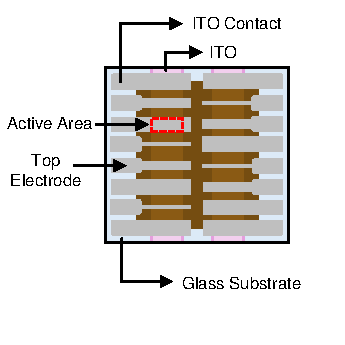
\includegraphics[width=\textwidth]{chapters/material_properties/images/Glass_Substrate.pdf} % Replace with your image
        \caption{Description for subplot (a).}
        \label{fig:ch2:glass_substrate}
    \end{subfigure}
    \hfill % Space between the two plots
    % Second plot
    \begin{subfigure}[t]{0.49\textwidth} % Adjust width as needed
        \centering
        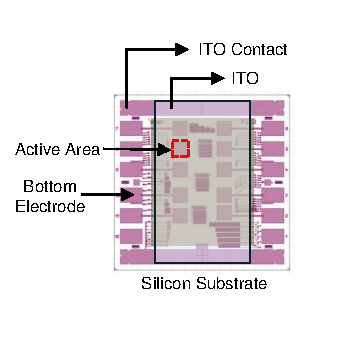
\includegraphics[width=\textwidth]{chapters/material_properties/images/PIX_Substrate.pdf} % Replace with your image
        \caption{Description for subplot (b).}
        \label{fig:ch2:pix_substrate}
    \end{subfigure}

    % Caption for the whole figure
    \caption{Comparison of experimentally measured and simulated Absorptance and Reflectance for the As-Deoisted and Annealed perovskite state.}
    \label{fig:ch2:types_of_substrates}
\end{figure}

\begin{figure}[htbp]
    \centering
    % First plot
    \begin{subfigure}[t]{0.49\textwidth} % Adjust width as needed
        \centering
        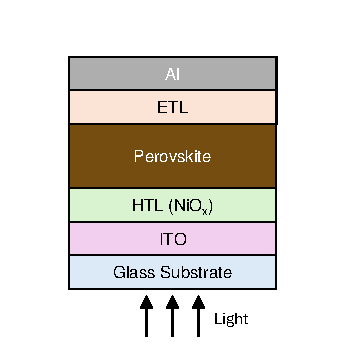
\includegraphics[width=\textwidth]{chapters/material_properties/images/Glass_Stack.pdf} % Replace with your image
        \caption{Description for subplot (a).}
        \label{fig:ch2:glass_stack}
    \end{subfigure}
    \hfill % Space between the two plots
    % Second plot
    \begin{subfigure}[t]{0.49\textwidth} % Adjust width as needed
        \centering
        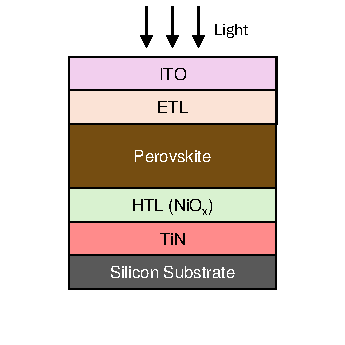
\includegraphics[width=\textwidth]{chapters/material_properties/images/PIX_Stack.pdf} % Replace with your image
        \caption{Description for subplot (b).}
        \label{fig:ch2:pix_stack}
    \end{subfigure}

    % Caption for the whole figure
    \caption{Comparison of experimentally measured and simulated Absorptance and Reflectance for the As-Deoisted and Annealed perovskite state.}
    \label{fig:ch2:types_of_stacks}
\end{figure}


\begin{itemize}
    \item Options for transport layers, deposition techniques and associated challenges, NiO always below the perovskite layer, explanation of NiO annealing effect on the conductivity of the perovskite layer
    \item Option for substrates (ITO - PIX), same stack, different source of light, masks and contacts
    \item Most important characterization for devices, specifications of figures of merit that are followed in this thesis, considerations on yield and statistical importance of the presented results
    \item (From Valdimir's thesis) Variations in the forward bias regime, device performance is very sensitive to small variations in resistance, it is not major focus in the work presented
\end{itemize}

\subsection{Impact of Characterization Method}

The characterization of perovskite0based deivces is not straightforward due to the fluid nature. Characterized by the presence of mobile ions, which follow that applied field an aprticipate at electrochemical reactios, which are partially reversible but there is a strong timeing element. 

This creates additioanl complications when electrically characterizing perovskite devices and espcially when comparing with literature. 

For the most standard scans, which are the most commonly performance ones, shows the impact of scan direction, as well as the impact of the inegration time. Scan direction highly is associated with hysteresis, while the integration time, the dark current start fomr the same value, it goes lower fro the scans with longer integration. 

An alternative characterization is enabled by the Paios characterzation suite, which enebles the possibility of the pulsed characterization. for each bias steop,bias is applied lin a pulsed way which is defined by the pulse duration and the measurements duration. For this demonstration, the measurement duration was fixed to 50 ms, while the pulse duration was varied between 100 and 1200 ms. In this case, the hysteresis is eliminated, however, it is clear that the longer the pulse duration the lower the levels of dark current, as well as the higher the forward current.

As a last option, is the steady state measurement, wehre the bias i maintained for a prolonged period of time. Which is associated with a large drop in the current value withing the first 10s of seconds before being stabilizing. The intial crop wa found to not depend so much on mobile ions (thorugh temperature related measurements) but rather capacitive effects. Which again can be impacted by the setup between groups. At -2 V a rapid increase of the cark value is observed, which is related to the reverse-bias induced breakdown of the device and will be further discussed in chpater 4. 

The impact of characterization approach extends to the EQE values, as well. Show the results for two differenct devices fabricated on the same samples. The first one was measured at 0V, and then at -1 V. While the second one wa measured t 0V, -1 V, and -2V. For both cases, the response was measured again right after with not bias, and the response is signifivalty lower compared to the riginal measurerement. However, we allowed for a 5 minute relaxation period. It was enough for the sampls biased up to -1 V to recover its original behavior, however this was not the case for the sample up to -2 V to revcover its original behavior. 

This highlights the complexity aroung the characterzation of different samples. For the rest of the work, we mainly rely on forward scans for the JV cahracteristics and measure EQE from 0v -1V -2V wihout prvious bias and this order. 

Even though it is not opssible to idenitfy a global value, we believ that his way allows for a fair comparison between different samples, empasizing on the trend of the impact of different modifications roather than absolute values.

Another point is related to the fair representation of J-V data. 12 devices are fabricated on the same sample. Usually there are a few outliers, whose number idenifies the variability in device perforamcne. Instead of selecting a more representative curve, which unavoidanty introduces the bias to the representation of the data, we opt for presenting a more staticitcal approach, as shown in Fig. The solid lines represents the median value and the shaded are respresent the interquartile range. This way, if there are only 1 or 2 outliers, they don't show up in the statistical represntatin, while if a large valriablity is oberved, it is tranlated into a very wide interquartile range.  

For example, fig xx showd

Additiaonlly, the fabrcaiton tools were used for mutliple activities within the group and there were periods of idle from recovered operation. These fluctuations from time to time had a big impact on the device peroformance, it was goal to establish a baseline performance. This means similr stacks, fabricated withing different phases of the phd might exhbiti small viariaontions. This is why when drawing comparisons, we only compare samples that were fabricated in close proximitiy to each other, to prevent un-fair comparisons with older better verisions of the same samples. 

\begin{figure}[htbp]
    \centering

    % First row
    \begin{subfigure}[b]{0.45\textwidth}
        \centering
        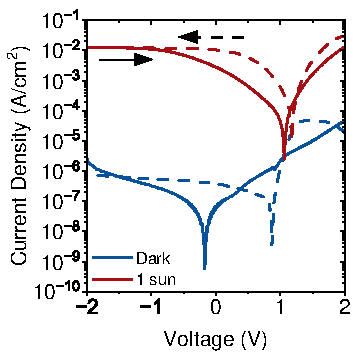
\includegraphics[width=\textwidth]{chapters/material_properties/images/Forward-Reverse-Plot.pdf}
        \caption{Figure 1}
    \end{subfigure}
    \hfill
    \begin{subfigure}[b]{0.45\textwidth}
        \centering
        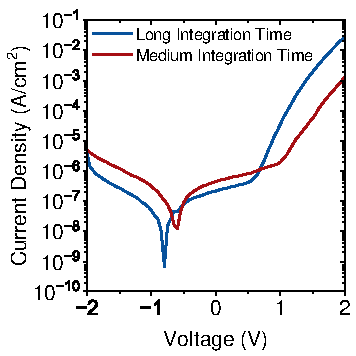
\includegraphics[width=\textwidth]{chapters/material_properties/images/Integration-Speed.pdf}
        \caption{Figure 2}
    \end{subfigure}

    \vspace{1em} % Space between rows

    % Second row
    \begin{subfigure}[b]{0.35\textwidth}
        \centering
        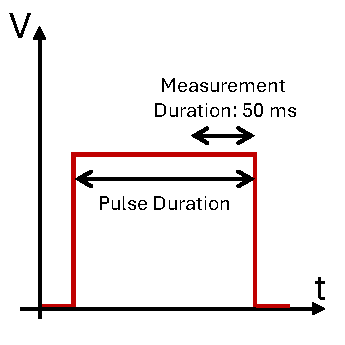
\includegraphics[width=\textwidth]{chapters/material_properties/images/PAIOS_Pulsed_Measurement.pdf}
        \caption{Figure 3}
    \end{subfigure}
    \hfill
    \begin{subfigure}[b]{0.45\textwidth}
        \centering
        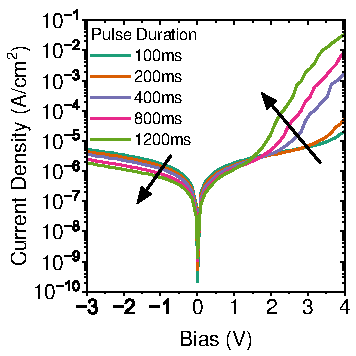
\includegraphics[width=\textwidth]{chapters/material_properties/images/Pulsed-PAIOS-plot.pdf}
        \caption{Figure 4}
    \end{subfigure}

    \vspace{1em} % Space between rows

    % Third row - centered figure
    \begin{subfigure}[b]{0.45\textwidth}
        \centering
        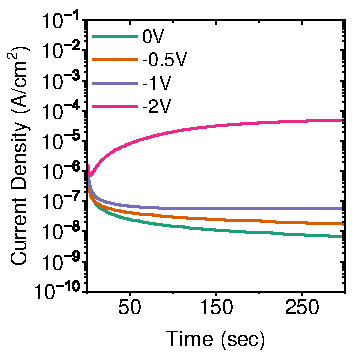
\includegraphics[width=\textwidth]{chapters/material_properties/images/Steady-State-plot.pdf}
        \caption{Figure 5}
    \end{subfigure}

    \caption{A figure with 3 rows: two rows of two images and one centered image.}
    \label{fig:three_rows}
\end{figure}


\begin{figure}[htbp]
    \centering
    % First plot
    \begin{subfigure}[t]{0.45\textwidth} % Adjust width as needed
        \centering
        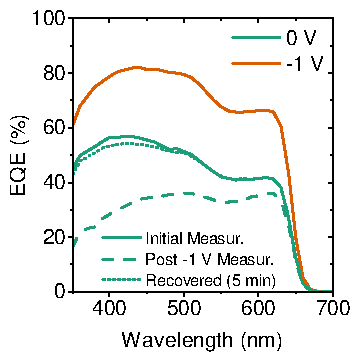
\includegraphics[width=\textwidth]{chapters/material_properties/images/EQE-1V.pdf} % Replace with your image
        \caption{Description for subplot (a).}
        \label{fig:ch2:eqe-1V}
    \end{subfigure}
    \hfill % Space between the two plots
    % Second plot
    \begin{subfigure}[t]{0.45\textwidth} % Adjust width as needed
        \centering
        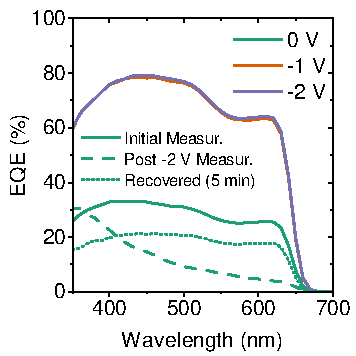
\includegraphics[width=\textwidth]{chapters/material_properties/images/EQE-2V.pdf} % Replace with your image
        \caption{Description for subplot (b).}
        \label{fig:ch2:eqe-2V}
    \end{subfigure}

    % Caption for the whole figure
    \caption{Comparison of experimentally measured and simulated Absorptance and Reflectance for the As-Deoisted and Annealed perovskite state.}
    \label{fig:ch2:eqe}
\end{figure}



\begin{figure}[htbp]
    \centering
    % First row
    \begin{subfigure}[t]{0.45\textwidth}
        \centering
        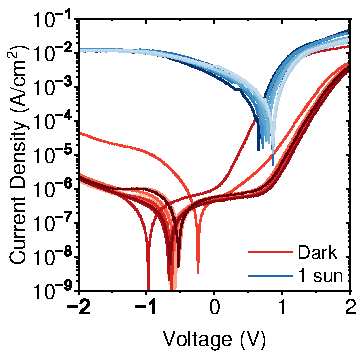
\includegraphics[width=\textwidth]{chapters/material_properties/images/High_yield_discrete.pdf} 
        \caption{}
        \label{fig:ch2:high_yield_discrete}
    \end{subfigure}
    \hfill
    \begin{subfigure}[t]{0.45\textwidth}
        \centering
        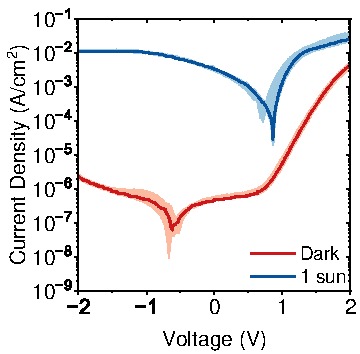
\includegraphics[width=\textwidth]{chapters/material_properties/images/High_yield_median.pdf} % Replace with your image file
        \caption{}
        \label{fig:ch2:high_yield_median}
    \end{subfigure}

    \vspace{1em} % Space between rows

    % Second row
    \begin{subfigure}[t]{0.45\textwidth}
        \centering
        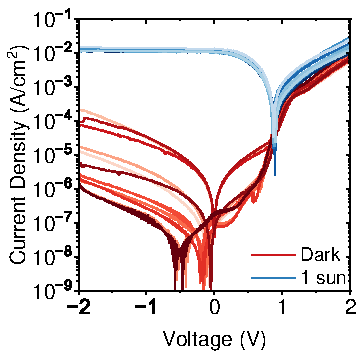
\includegraphics[width=\textwidth]{chapters/material_properties/images/low_yield_discrete.pdf} % Replace with your image file
        \caption{}
        \label{fig:ch2:low_yield_discrete}
    \end{subfigure}
    \hfill
    \begin{subfigure}[t]{0.45\textwidth}
        \centering
        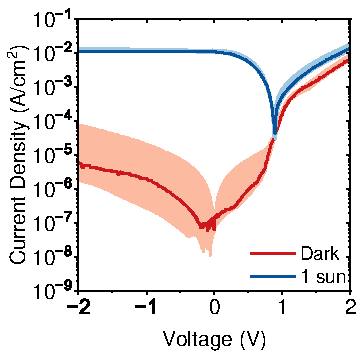
\includegraphics[width=\textwidth]{chapters/material_properties/images/low_yield_median.pdf} % Replace with your image file
        \caption{}
        \label{fig:ch2:low_yield_median}
    \end{subfigure}
    \caption{SSPL, TRPL, and absorptance for the an As-Deposited and an Annealed perovskite sample.}
\end{figure}



\subsection{Impact of Electron Transport Layer}

One of the first step was to compare the performance of the as-deposited and annealed PePD, using two different ETLs, the main ones that were investigarted in the framework of this study, e-beam deposited TiO2 and thermally evaporated C60. the forward scans for TiO2 samples and c60 ones, are shown in Fig. xx and yy respetively. For TiO2, both deivces have similar performance , the annealed sample shows a smaller hysteresis. the median dark current at -2V varies between 0.7 mA.cm2 and 10 uA/cm2. The perofromance is not the same with c60. Both samples show significantly higher levels of Jd, with the as-deposited samples having a migh larger spread. This will be furthe investgated on the chapter about the optimization of the ETL, but is mainly attributed to the abundand grain bonaries of the as-deposited samples, the diffusion of C60 trhough them and the creating of metalling shorts. This is partially mitigated fot the annealed sample, which has significantly larger grain size but is not completerly eliminated. 

In terms of EQE for the Tio2 samples, both as-deposited and annealed sample ehibit a similar behavior with an EQE that saturates even at 0V and is mainly above 70 \% for the whole visible range. This further highlights the possiblity of farbircating all-evaporated devices at complete room tempreature, further extensions for substrates and requires applications that need black phase at room temperature. Howver, considering the improvements in crystallinity and reduction in non-radiative recombination that were established for the annealed state, we move forward using the f;ash-annealed sample with 40 nm of TiO2 as the baseline. 




\begin{figure}[htbp]
    \centering
    % First row
    \begin{subfigure}[t]{0.45\textwidth}
        \centering
        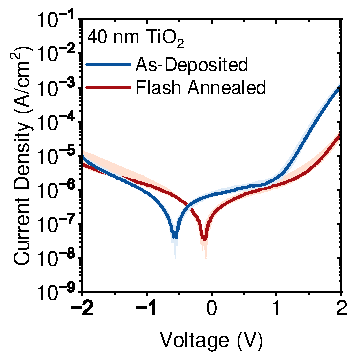
\includegraphics[width=\textwidth]{chapters/material_properties/images/TiO2-Compare.pdf} 
        \caption{}
        \label{fig:ch2:tio2_compare}
    \end{subfigure}
    \hfill
    \begin{subfigure}[t]{0.45\textwidth}
        \centering
        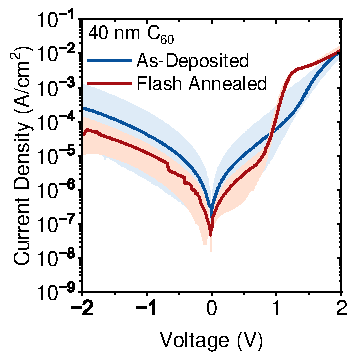
\includegraphics[width=\textwidth]{chapters/material_properties/images/C60-Compare.pdf} % Replace with your image file
        \caption{}
        \label{fig:ch2:c60_compare}
    \end{subfigure}

    \vspace{1em} % Space between rows

    % Second row
    \begin{subfigure}[t]{0.45\textwidth}
        \centering
        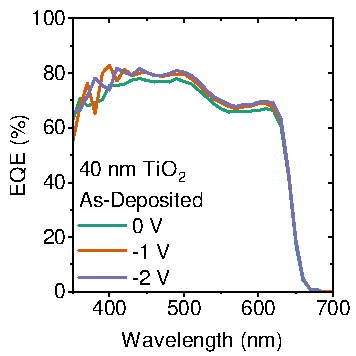
\includegraphics[width=\textwidth]{chapters/material_properties/images/As_Dep-EQE.pdf} % Replace with your image file
        \caption{}
        \label{fig:ch2:as_dep_eqe}
    \end{subfigure}
    \hfill
    \begin{subfigure}[t]{0.45\textwidth}
        \centering
        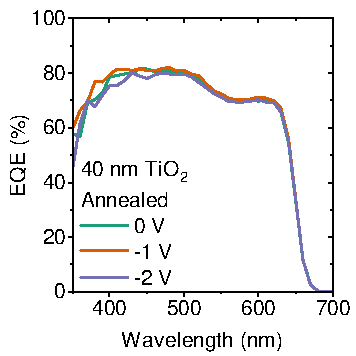
\includegraphics[width=\textwidth]{chapters/material_properties/images/Annealed_EQE.pdf} % Replace with your image file
        \caption{}
        \label{fig:ch2:annealed_eqe}
    \end{subfigure}
    \caption{SSPL, TRPL, and absorptance for the an As-Deposited and an Annealed perovskite sample.}
\end{figure}


\subsection{Impact of Perovskite Deposition Conditions}

\begin{itemize}
    \item Part on defect tolerance of the perovskite layer and its implications on the tolerance against changes in the device characteristics by changing deposition consitions
    \item Impact of deposition rate, ratio between precursors, annealing duration
    \item Exploration of 3-source evaporation of CsPbI2Br films and the problems with pinholes and shunts in device performance. 
\end{itemize}

\begin{figure}[htbp]
    \centering
    % First row
    \begin{subfigure}[t]{0.45\textwidth}
        \centering
        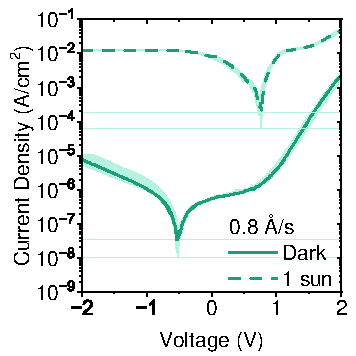
\includegraphics[width=\textwidth]{chapters/material_properties/images/08As-JV.pdf} 
        \caption{}
        \label{fig:ch2:0.8A/s-jv}
    \end{subfigure}
    \hfill
    \begin{subfigure}[t]{0.45\textwidth}
        \centering
        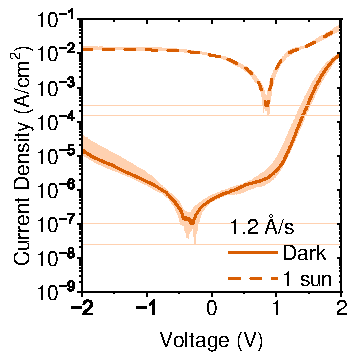
\includegraphics[width=\textwidth]{chapters/material_properties/images/12AS-JV.pdf} % Replace with your image file
        \caption{}
        \label{fig:ch2:1.2A/s-vj}
    \end{subfigure}

    \vspace{1em} % Space between rows

    % Second row
    \begin{subfigure}[t]{0.45\textwidth}
        \centering
        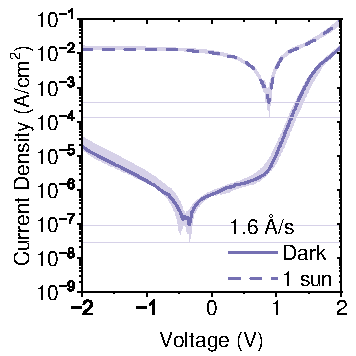
\includegraphics[width=\textwidth]{chapters/material_properties/images/16AS-JV.pdf} % Replace with your image file
        \caption{}
        \label{fig:ch2:1.6A/s-jv}
    \end{subfigure}
    \hfill
    \begin{subfigure}[t]{0.45\textwidth}
        \centering
        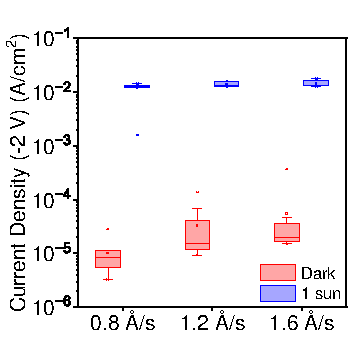
\includegraphics[width=\textwidth]{chapters/material_properties/images/Evap_Rate_Box_Plot.pdf} % Replace with your image file
        \caption{}
        \label{fig:ch2:box_plot_evap_rate}
    \end{subfigure}
    \caption{SSPL, TRPL, and absorptance for the an As-Deposited and an Annealed perovskite sample.}
\end{figure}




\begin{figure}[htbp]
    \centering

    % First row
    \begin{subfigure}[b]{0.3\textwidth}
        \centering
        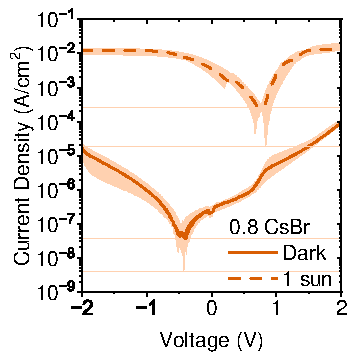
\includegraphics[width=\textwidth]{chapters/material_properties/images/08CsBr.pdf}
        \caption{Figure 1}
    \end{subfigure}
    \hfill
    \begin{subfigure}[b]{0.3\textwidth}
        \centering
        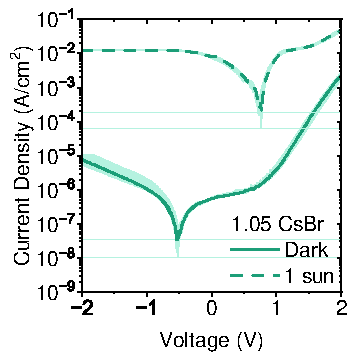
\includegraphics[width=\textwidth]{chapters/material_properties/images/105CsBr.pdf}
        \caption{Figure 2}
    \end{subfigure}
    \hfill
    \begin{subfigure}[b]{0.3\textwidth}
        \centering
        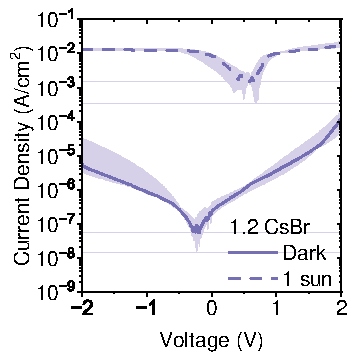
\includegraphics[width=\textwidth]{chapters/material_properties/images/12CsBr.pdf}
        \caption{Figure 3}
    \end{subfigure}

    \vspace{1em} % Space between rows

    % Second row
    \begin{subfigure}[b]{0.3\textwidth}
        \centering
        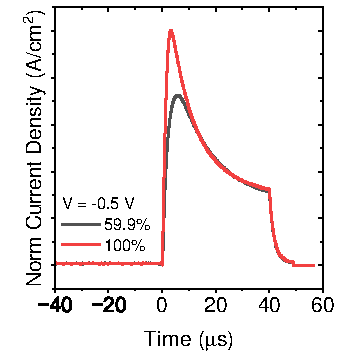
\includegraphics[width=\textwidth]{chapters/material_properties/images/TPC-08CsBr.pdf}
        \caption{Figure 4}
    \end{subfigure}
    \hfill
    \begin{subfigure}[b]{0.3\textwidth}
        \centering
        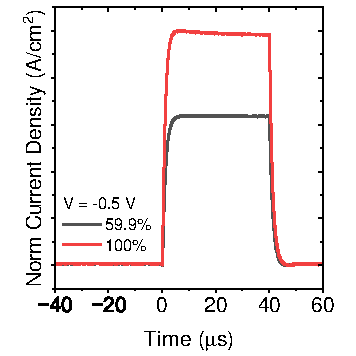
\includegraphics[width=\textwidth]{chapters/material_properties/images/TPC-105CsBr.pdf}
        \caption{Figure 5}
    \end{subfigure}
    \hfill
    \begin{subfigure}[b]{0.3\textwidth}
        \centering
        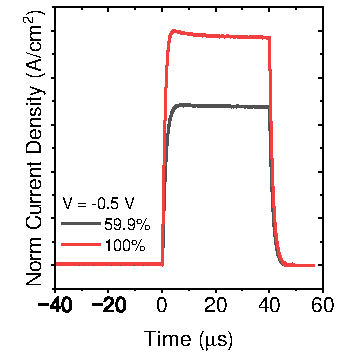
\includegraphics[width=\textwidth]{chapters/material_properties/images/tpc-12CsBr.pdf}
        \caption{Figure 6}
    \end{subfigure}

    \caption{A figure with 2 rows and 3 images in each row.}
    \label{fig:two_rows_three_columns}
\end{figure}




\subsection{Impact of Substrate}

\begin{itemize}
    \item Comparison of JVs and EQE between glass/ITO and PIX 
    \item Explanation of the higher resistivity of the PIX substrates through the TEM submitted samples
    \item Proof of the high-temperature stability of the stack through annealing of the complete PIX stack post-depositions
    \item Only possible to evaluate for PIX and not for Al, since it will diffuse in the stack 
\end{itemize}


\begin{figure}[h!]
    \centering
    % First row: Two figures
    \begin{minipage}{0.48\textwidth}
        \centering
        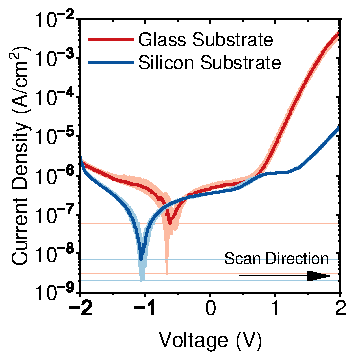
\includegraphics[width=\textwidth]{chapters/material_properties/images/JV_PIX_Glass.pdf} % Replace with your file
        \caption{Figure 1 Caption}
        \label{fig:ch2:jv_comp_pic_glass}
    \end{minipage}
    \hfill
    \begin{minipage}{0.48\textwidth}
        \centering
        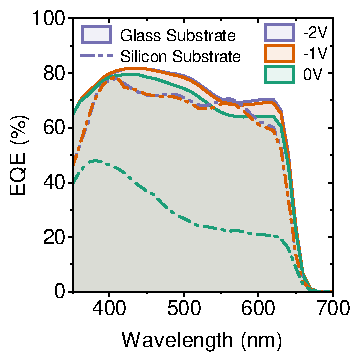
\includegraphics[width=\textwidth]{chapters/material_properties/images/EQE_fnm_PIX_Glass.pdf} % Replace with your file
        \caption{Figure 2 Caption}
        \label{fig:ch2:eqe_comp_pix_glass}
    \end{minipage}

    % Second row: One figure
    \vspace{1em} % Adjust vertical space
    \begin{minipage}{0.48\textwidth}
        \centering
        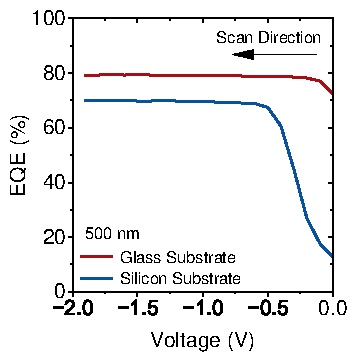
\includegraphics[width=\textwidth]{chapters/material_properties/images/EQE_fV_PIX_Glass.pdf} % Replace with your file
        \caption{Figure 3 Caption}
        \label{fig:ch2:eqefV_comp_pix_glass}
    \end{minipage}
\end{figure}







\begin{figure}[htbp]
    \centering
    % First row
    \begin{subfigure}[t]{0.49\textwidth}
        \centering
        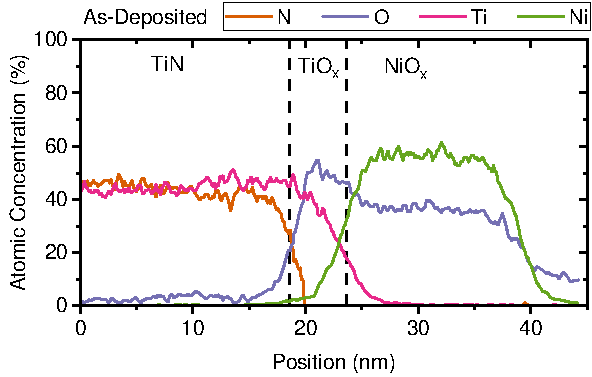
\includegraphics[width=\textwidth]{chapters/material_properties/images/TEM_As_Dep.pdf} % Replace with your image file
        \caption*{(a)}
    \end{subfigure}
    \hfill
    \begin{subfigure}[t]{0.49\textwidth}
        \centering
        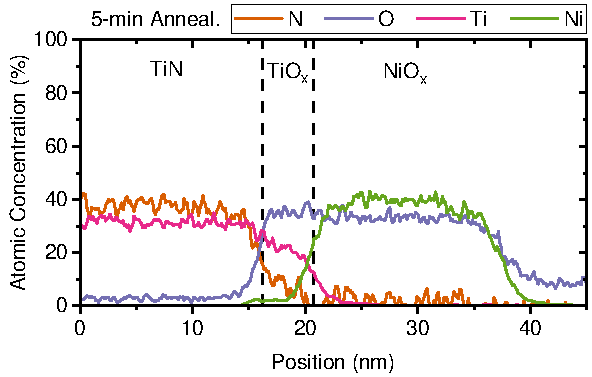
\includegraphics[width=\textwidth]{chapters/material_properties/images/TEM_5_min.pdf} % Replace with your image file
        \caption*{(b)}
    \end{subfigure}

    \vspace{1em} % Space between rows

    % Second row
    \begin{subfigure}[t]{0.49\textwidth}
        \centering
        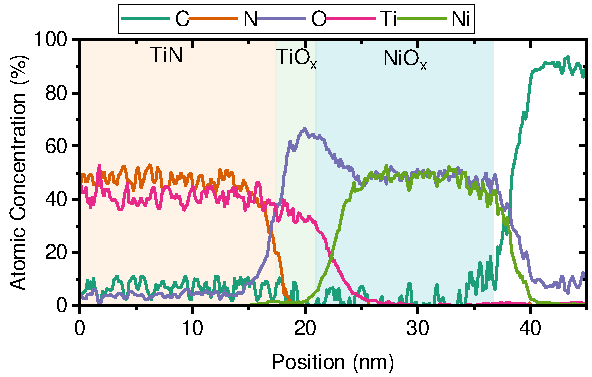
\includegraphics[width=\textwidth]{chapters/material_properties/images/TEM_30_min.pdf} % Replace with your image file
        \caption*{(c)}
    \end{subfigure}
    \hfill
    \begin{subfigure}[t]{0.49\textwidth}
        \centering
        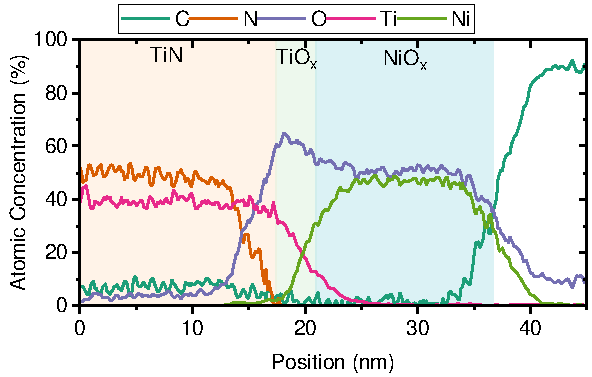
\includegraphics[width=\textwidth]{chapters/material_properties/images/TEM_60_min.pdf} % Replace with your image file
        \caption*{(d)}
    \end{subfigure}
    \caption{TEM of TiN - NiOx interface and emergence of TiOx at the interface.}
\end{figure}




%%%%%%%%%%%%%%%%%%%%%%%%%%%%%%%%%%%%%%%%%%%%%%%%%%
% Keep the following \cleardoublepage at the end of this file, 
% otherwise \includeonly includes empty pages.
\cleardoublepage

